\newpage
\section{Contributions}
\begin{table}[h]
\centering
\resizebox{\textwidth}{!}{\begin{tabular}{|l|llll|}
\hline
\textbf{Task} & \multicolumn{1}{l|}{\textbf{Amal Chandra}} & \multicolumn{1}{l|}{\textbf{Dylan Fu}} & \multicolumn{1}{l|}{\textbf{Quentin Heng}} & \multicolumn{1}{l|}{\textbf{Louis Pienaar}} \\ \hline
\textbf{Analogue Design} & 22\% & 34\% & 34\% & 10\%                                \\ \cline{1-1}
\textbf{Analogue Testing \& Verification} & 33\% & 33\% & 33\% & 1\%                  \\ \cline{1-1}
\textbf{Assembly} & 60\% & 20\% & 20\% & 0\%                                          \\ \cline{1-1}
\textbf{Path Algorithms} & 5\% & 12.5\% & 12.5\% & 70\%                                   \\ \cline{1-1}
\textbf{Benchmark Tests} & 25\% & 25\% & 25\% & 25\%                                    \\ \cline{1-1}
\textbf{Software Design} & 10\% & 15\% & 15\% & 60\%                                \\ \cline{1-1}
\textbf{Software Testing \& Verification} & 10\% & 25\% & 25\% & 40\%               \\ \cline{1-1}
\textbf{Integration} & 25\% & 25\% & 25\% & 25\%                                    \\ \cline{1-1}
\textbf{Report} & 25\% & 25\% & 25\% & 25\%                                       \\ \hline
\end{tabular}}
% \caption{Table of contributions towards the project}
\end{table}

\section{Appendices}
\subsection*{Appendix: A}
\begin{table}[h!]
\centering
\resizebox{\textwidth}{!}{\begin{tabular}{|l|l|l|l|l|l|l|}
\hline
\textbf{Photo-transistor Configuration}                  & \textbf{Type} & \textbf{Min} & \textbf{Max} & \textbf{Avg} & \textbf{Pk-Pk} & \textbf{Frequency} \\ \hline
\multirow{2}{*}{\textbf{Common Collector}} & \textbf{White} & $1.38V$ & $-1.31V$ & $0.06V$ & $2.13V$ & $120Hz$          \\ \cline{2-7} 
                           & \textbf{Black} & $0.92V$ & $-0.93V$ & $0.06V$ & $2.13V$ & $120Hz$          \\ \hline
\multirow{2}{*}{\textbf{Common Emitter}} & \textbf{White} & $3.7V$ & $1.93V$ & $3V$ & $1.8V$ &  $120Hz$         \\ \cline{2-7} 
                           & \textbf{Black} & $4.46V$ & $4.18V$ & $4.33V$ & $0.28V$ & $120Hz$          \\ \hline
\end{tabular}}
\caption{Voltage comparison using different photo-transistor configurations.}
\end{table}

\begin{table}[h!]
\centering
\resizebox{\textwidth}{!}{\begin{tabular}{|l|l|l|l|l|l|l|}
\hline
\textbf{Light Source}                  & \textbf{Type} & \textbf{Min} & \textbf{Max} & \textbf{Avg} & \textbf{Pk-Pk} & \textbf{Frequency} \\ \hline
\multirow{2}{*}{\textbf{Projector Only}} & \textbf{White} & $4.4V$ & $0.06V$ & $1.6V$ & $4.3V$ & $120Hz$          \\ \cline{2-7} 
                           & \textbf{Black} & $0.38V$ & $0.06V$ & $0.18V$ & $0.32V$ & $120Hz$          \\ \hline
\multirow{2}{*}{\textbf{All Lights On}} & \textbf{White} & $3.4V$ & $0.07V$ & $1.1V$ & $3.1V$ &  $120Hz$         \\ \cline{2-7} 
                           & \textbf{Black} & $0.54V$ & $0.06V$ & $0.02V$ & $0.48V$ & $120Hz$          \\ \hline
\end{tabular}}
\caption{Voltage comparison between black and white light.}
\end{table}

\begin{table}[h!]
\centering
\resizebox{\textwidth}{!}{\begin{tabular}{|l|l|l|l|l|l|l|}
\hline
\textbf{} & \multicolumn{2}{l|}{\textbf{Array}}           & \multicolumn{2}{l|}{\textbf{Linked List}}           & \multicolumn{2}{l|}{\textbf{Queue}}           \\\hline
\textbf{Situation} & \textit{\textbf{Average}} & \textit{\textbf{Worst}} & \textit{\textbf{Average}} & \textit{\textbf{Worst}} & \textit{\textbf{Average}} & \textit{\textbf{Worst}} \\\hline
\textbf{Accessing Element} & $O(1)$ & $O(n)$ & $O(n)$ & $O(n)$ & $O(n)$ & $O(n)$ \\\hline
\textbf{Insertion/Deletion} & $O(n)$ & $O(n)$ & $O(1)$ & $O(1)$ & $O(1)$ &  $O(1)$ \\\hline         
\end{tabular}}
\caption{Time complexity comparison between arrays, linked lists and queues.}
\end{table}

\newpage
\subsection*{Appendix: B}
\begin{multicols}{2}

\begin{figure}[H]
\centering
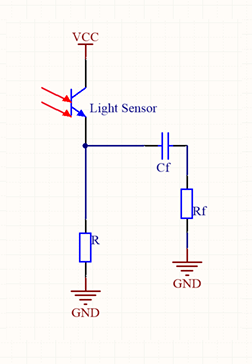
\includegraphics[width=0.4\textwidth]{figures/common-collector}
\caption{Common Collector configuration of the light sensor.}
\end{figure}

\begin{figure}[H]
\centering
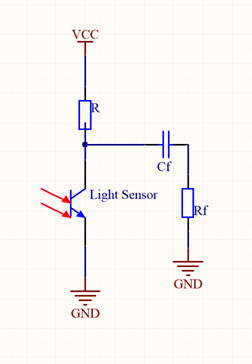
\includegraphics[width=0.4\textwidth]{figures/common-emitter.png}
\caption{Common Emitter configuration of the light sensor.}
\end{figure}
\end{multicols}

\begin{figure}[H]
\centering
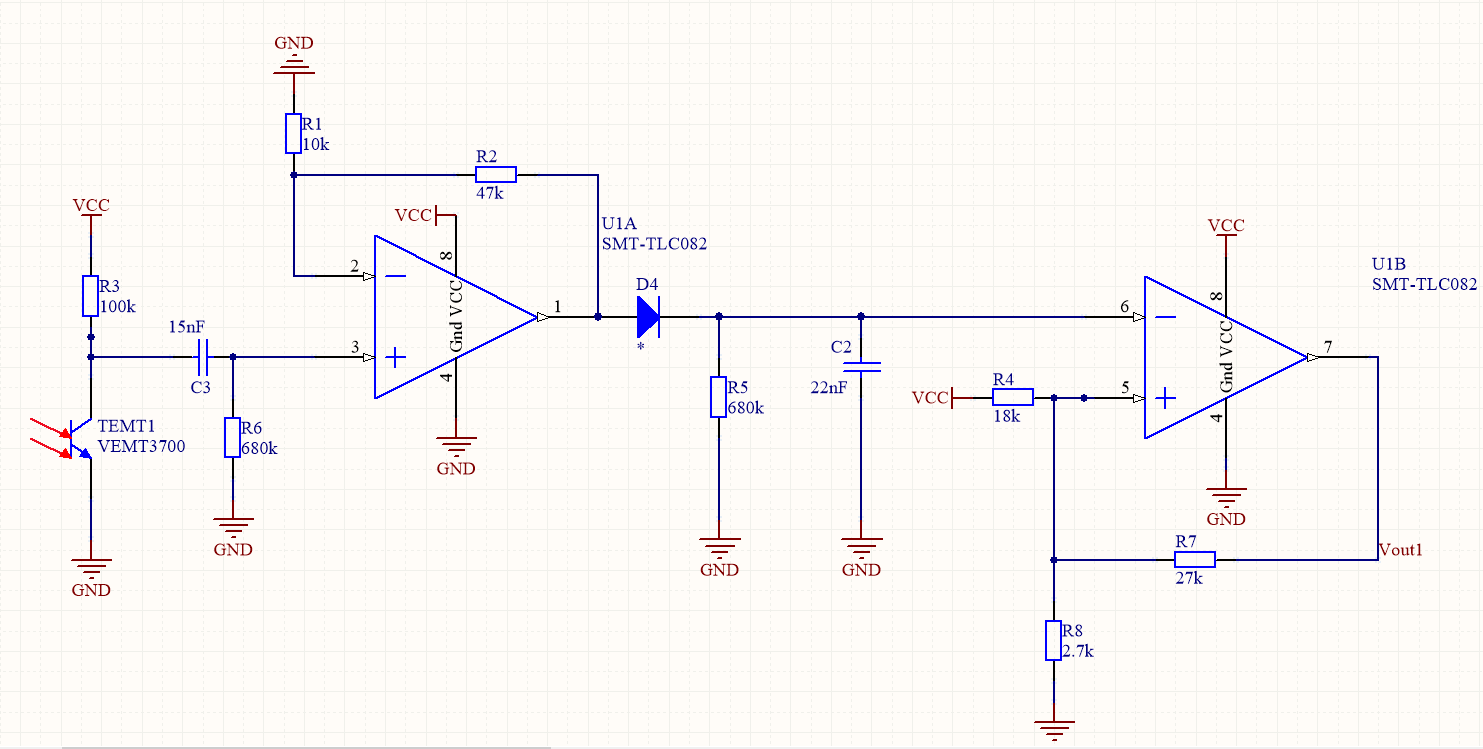
\includegraphics[width=\textwidth]{figures/full-circuit.png}
\caption{Final light sensing circuit design.}
\end{figure}

\subsection*{Appendix: C}

\begin{figure}[H]
\centering
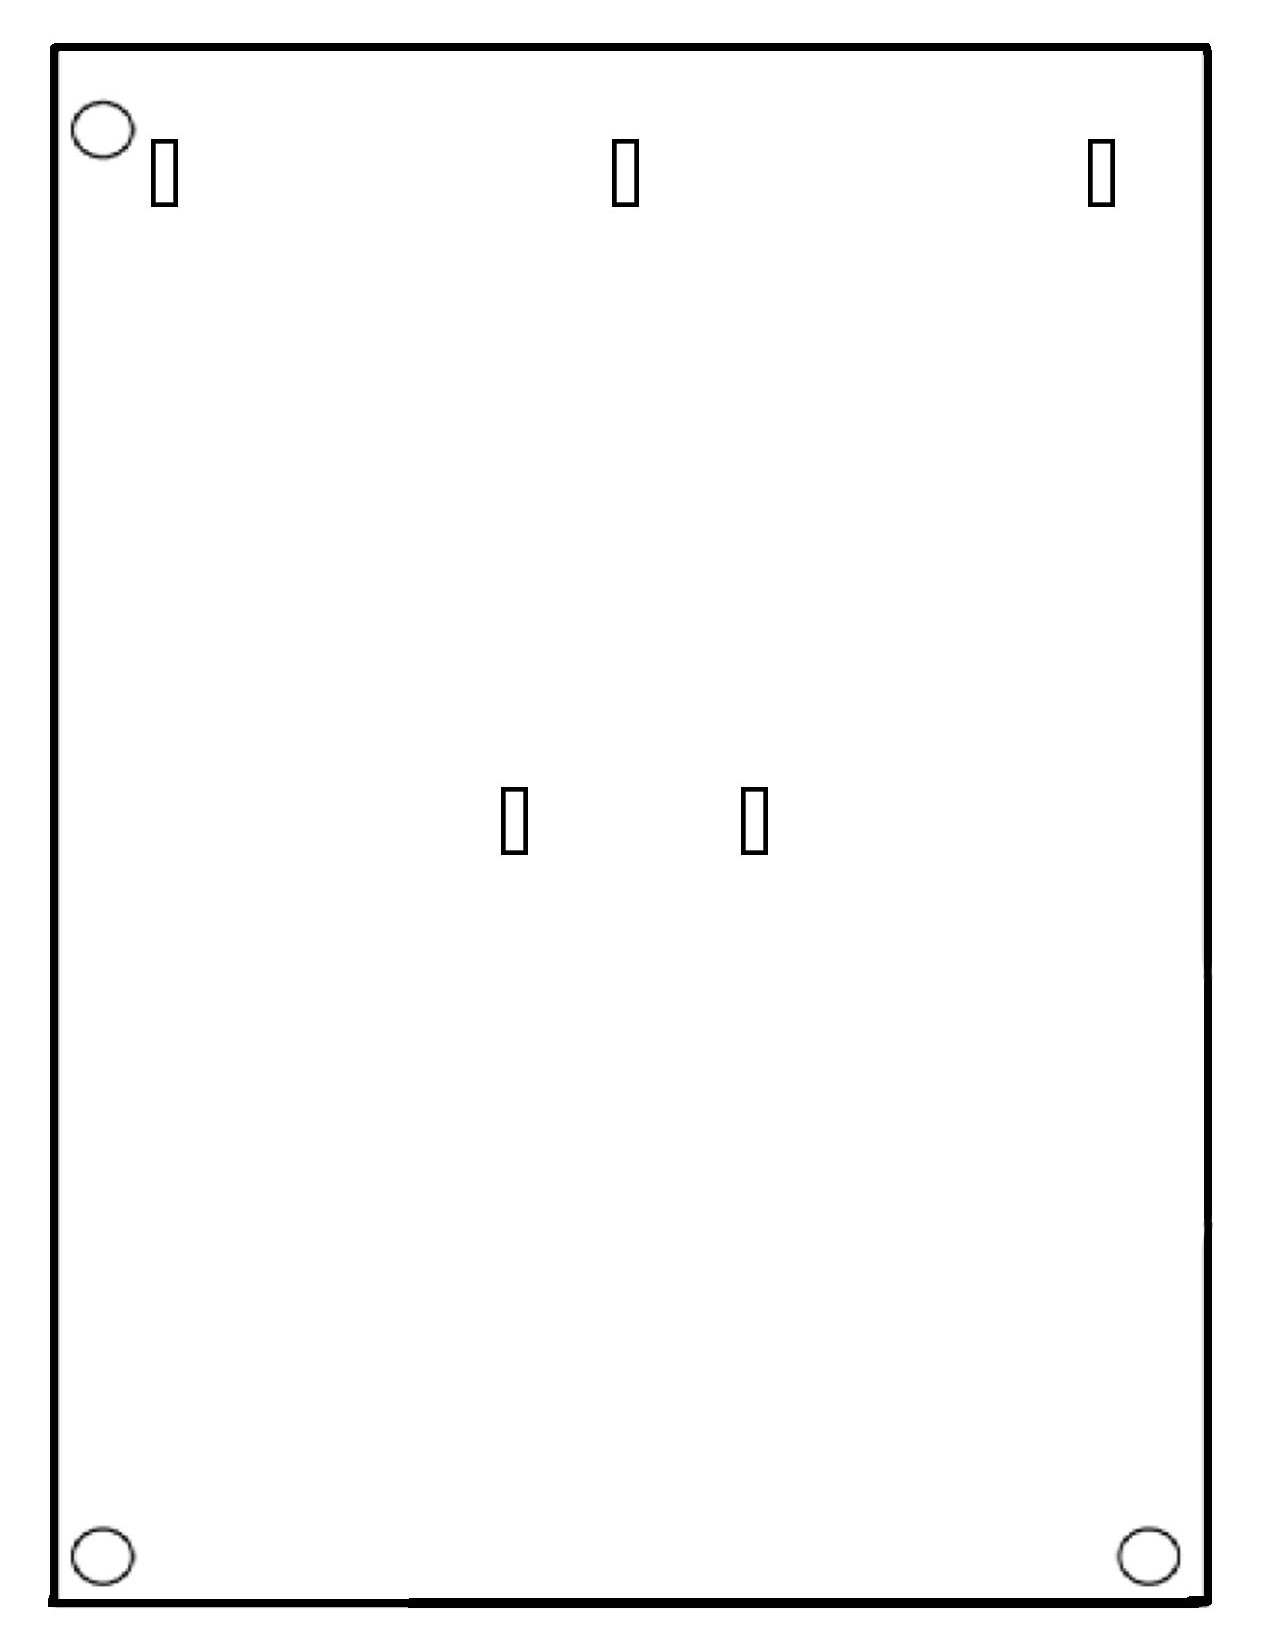
\includegraphics[width=0.95\textwidth]{figures/sarray1.jpg}
\caption{Sensor Arrangement 1.}
\end{figure}


\begin{figure}[H]
\centering
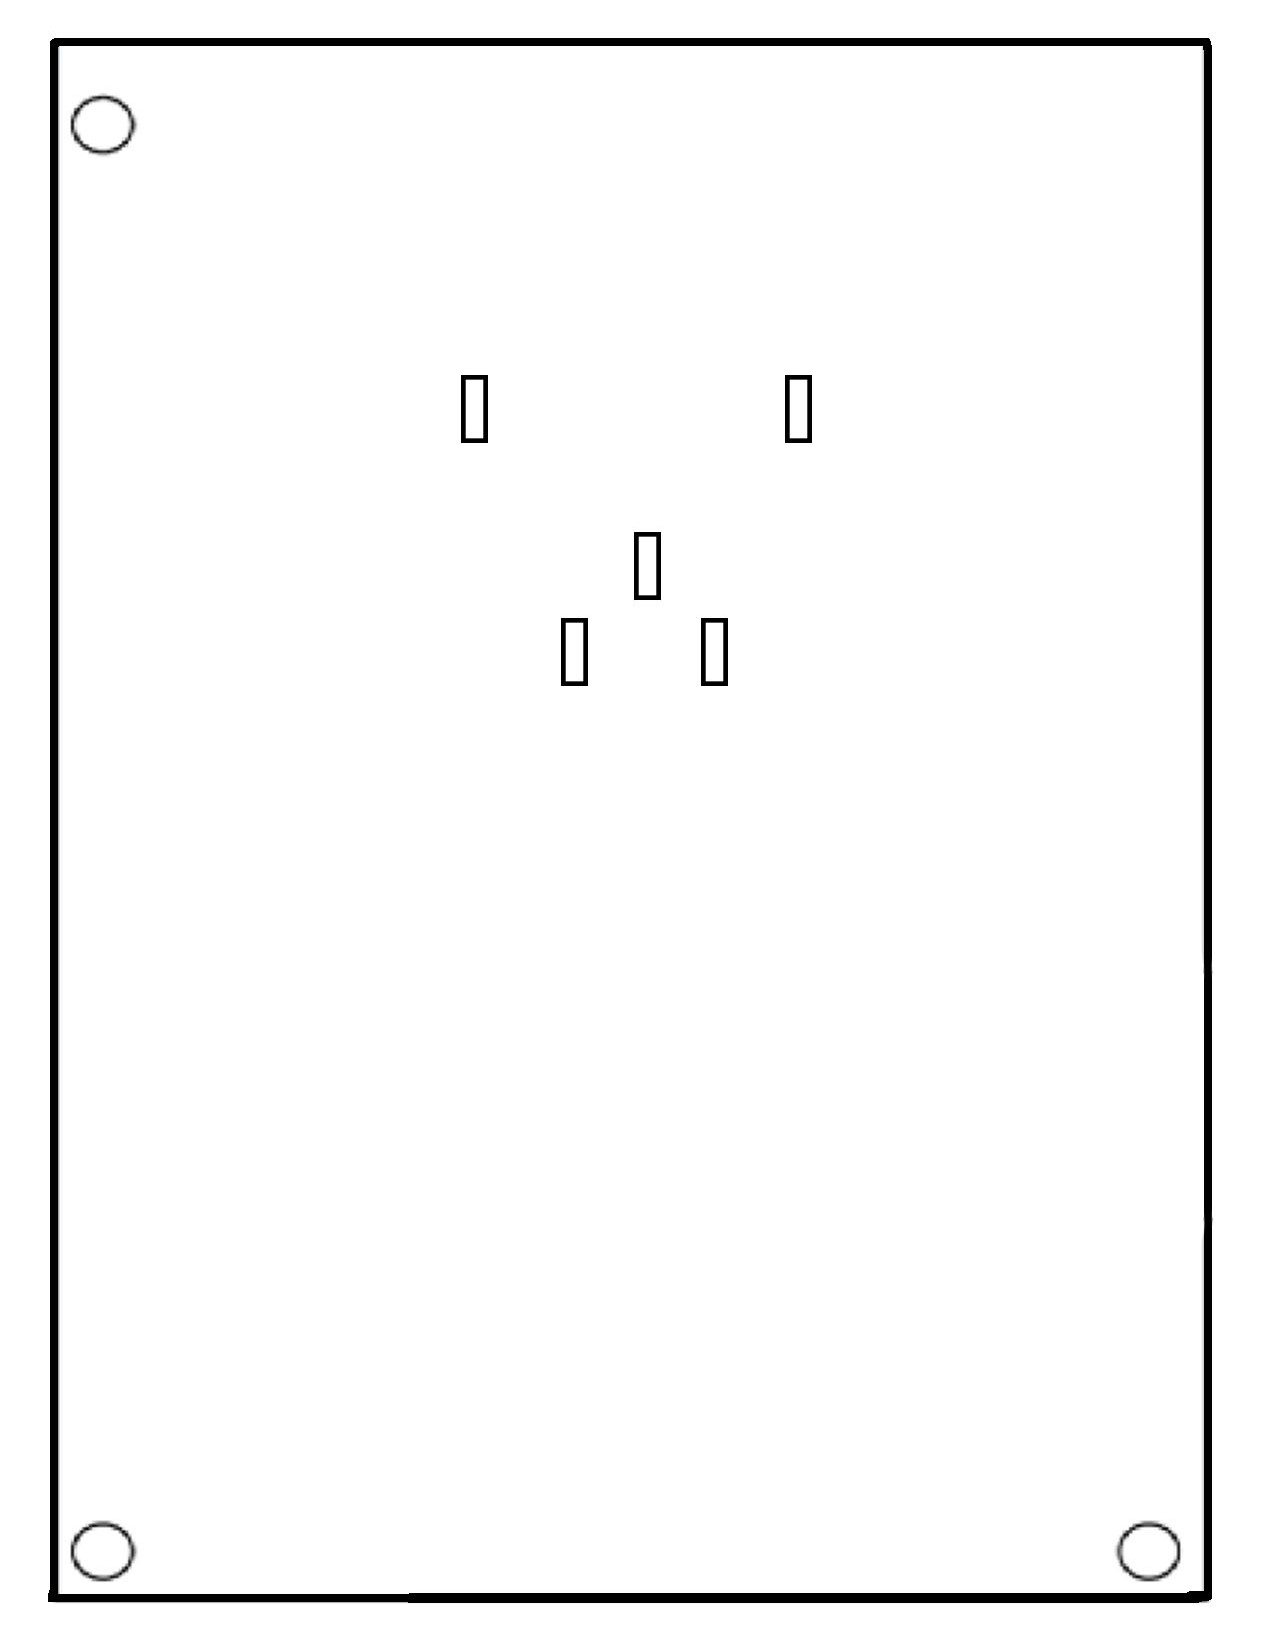
\includegraphics[width=0.95\textwidth]{figures/sarray2.jpg}
\caption{Sensor Arrangement 2.}
\end{figure}

\begin{figure}[H]
\centering
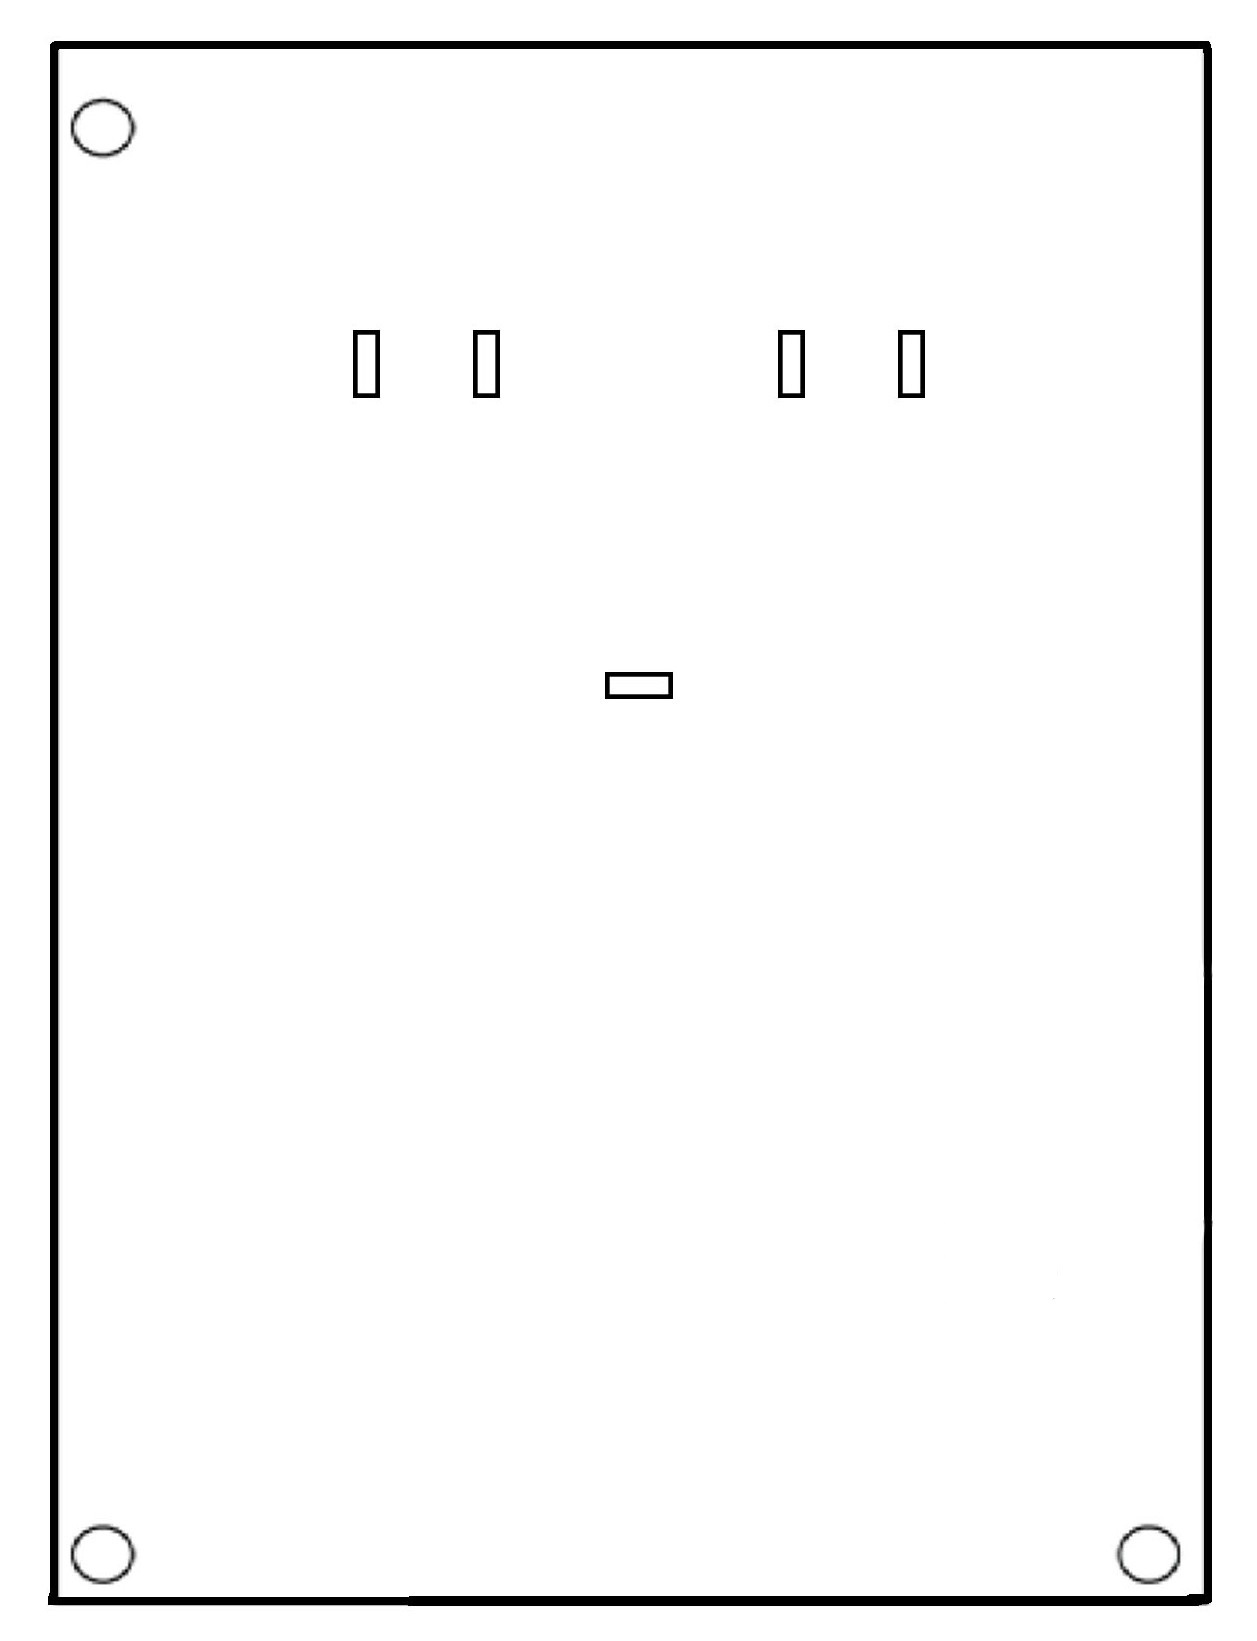
\includegraphics[width=0.95\textwidth]{figures/sarray3.jpg}
\caption{Final Sensor Arrangement.}
\end{figure}

\newpage
\subsection*{Appendix: D}

\begin{multicols}{2}

\begin{figure}[H]
\centering
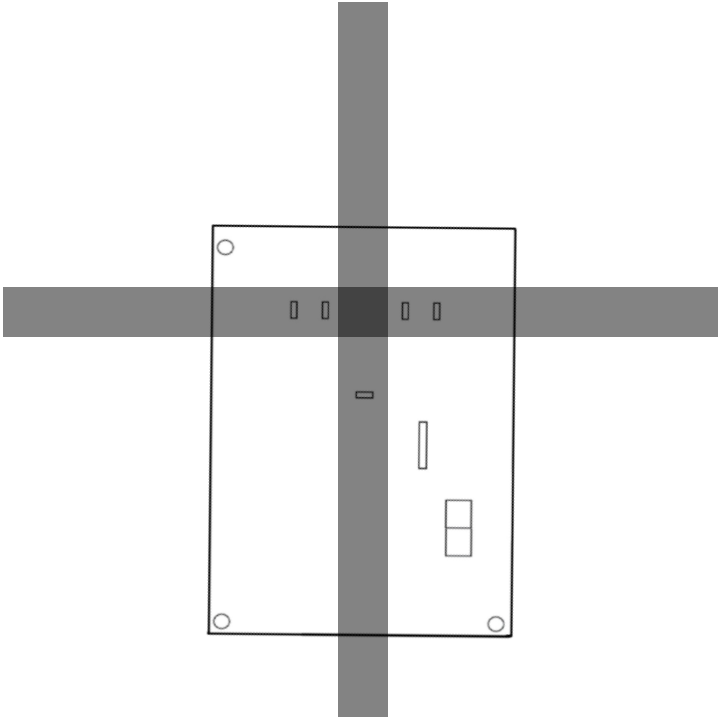
\includegraphics[width=0.3\textwidth]{figures/intersection-1.png}
\caption{Event detected by both Intersection Sensors.}
\end{figure}

\begin{figure}[H]
\centering
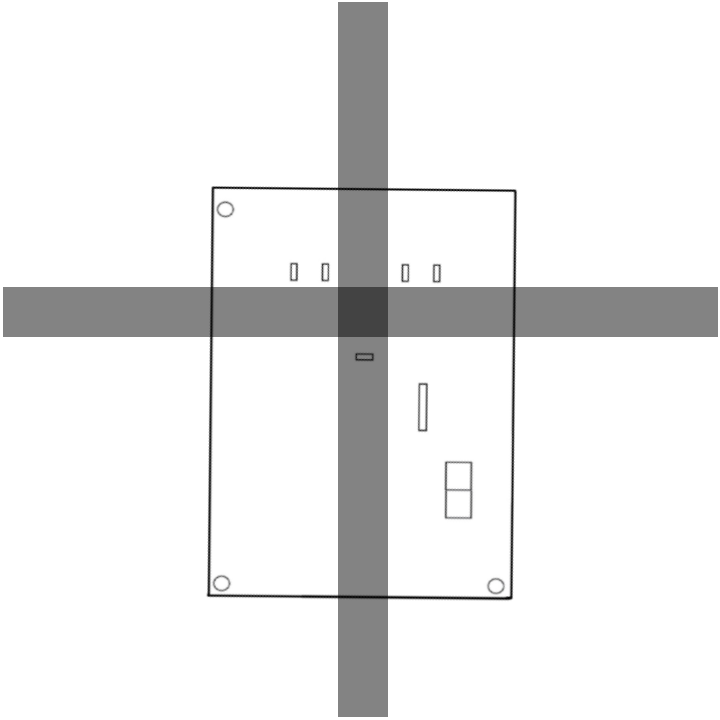
\includegraphics[width=0.3\textwidth]{figures/intersection-2.png}
\caption{Event detection finished, robot will perform appropriate action.}
\end{figure}

\end{multicols}

\begin{multicols}{4}

\begin{figure}[H]
\centering
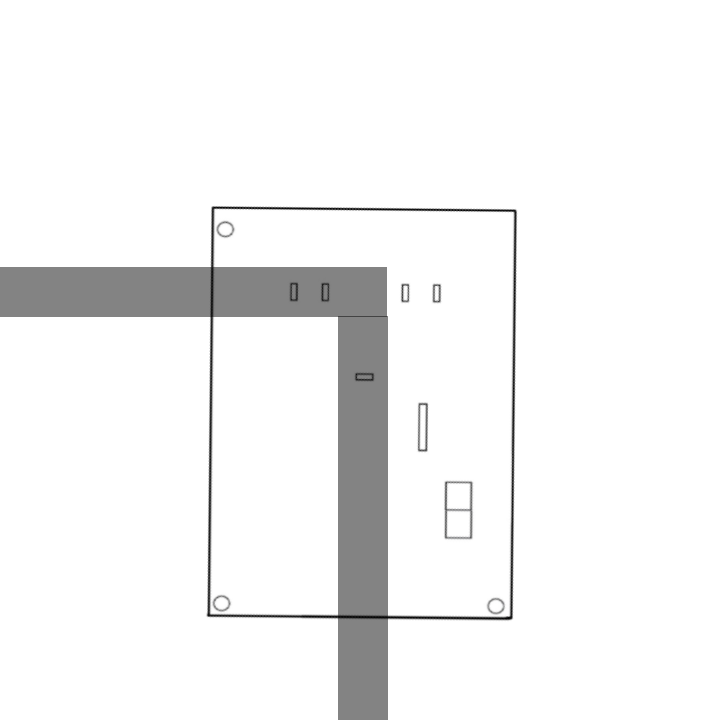
\includegraphics[width=0.2\textwidth]{figures/corner-1.png}
\caption{Event detected by left intersection sensor. Left corner inferred based on internal logic.}
\end{figure}

\begin{figure}[H]
\centering
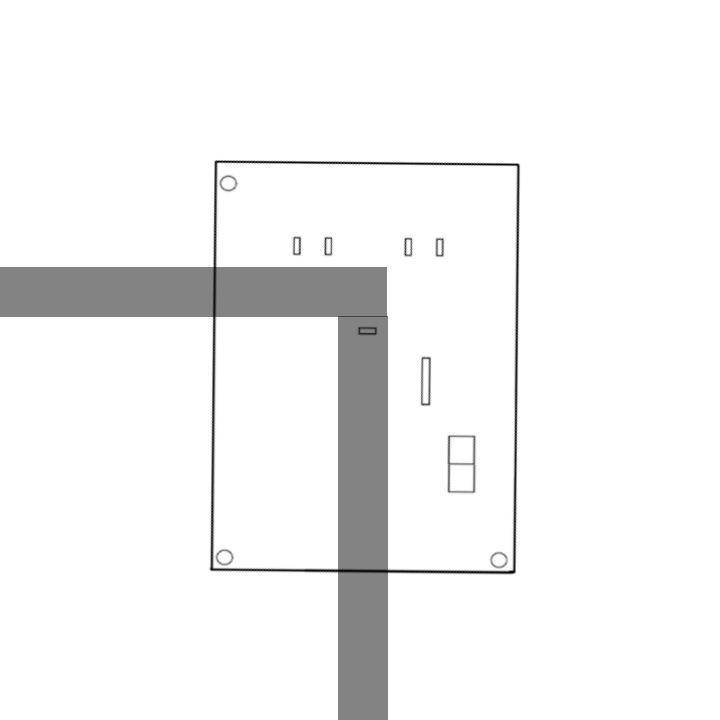
\includegraphics[width=0.2\textwidth]{figures/corner-2.png}
\caption{Event detection finished. Robot will perform appropriate action.}
\end{figure}

\begin{figure}[H]
\centering
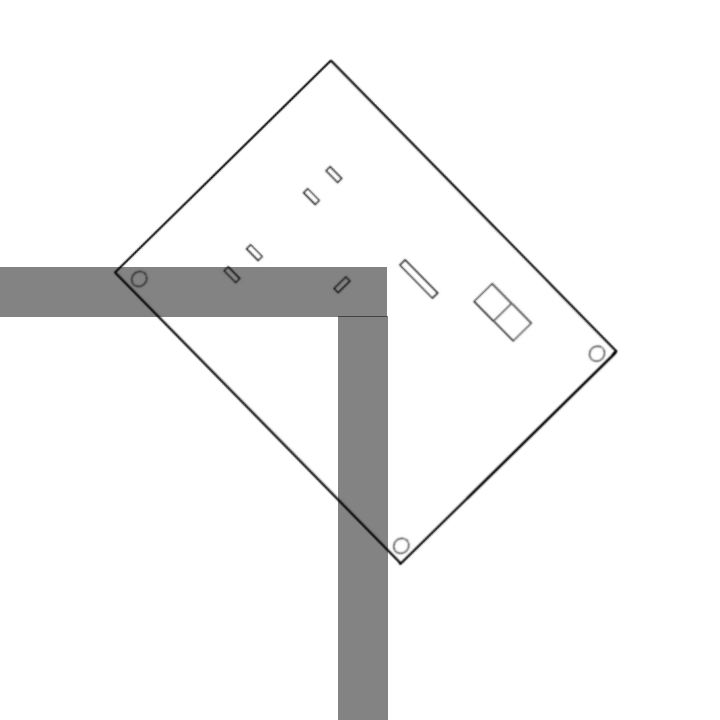
\includegraphics[width=0.2\textwidth]{figures/corner-3.png}
\caption{Robot begins turning here.}
\end{figure}

\begin{figure}[H]
\centering
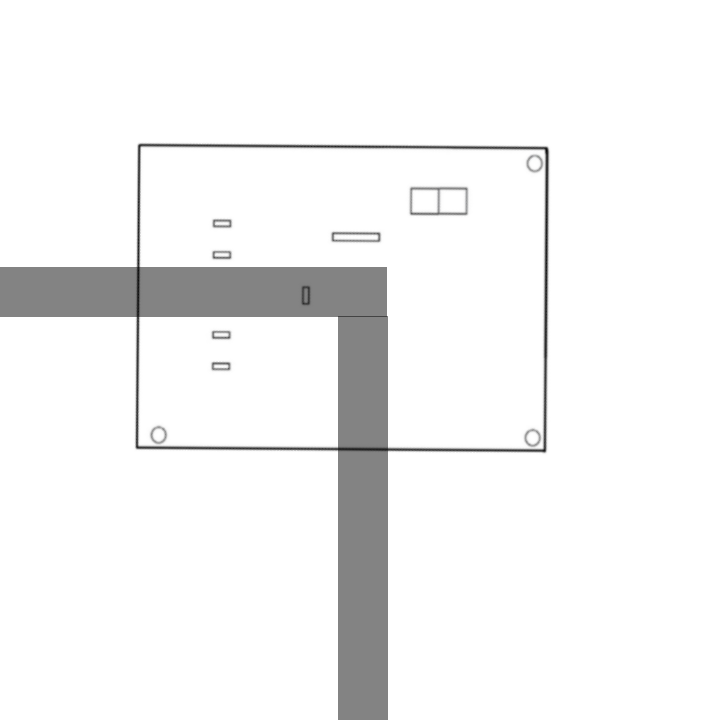
\includegraphics[width=0.2\textwidth]{figures/corner-4.png}
\caption{Robot completes turn. Light sensor return to neutral state.}
\end{figure}

\end{multicols}

\vspace{4mm}

\begin{multicols}{4}

\begin{figure}[H]
\centering
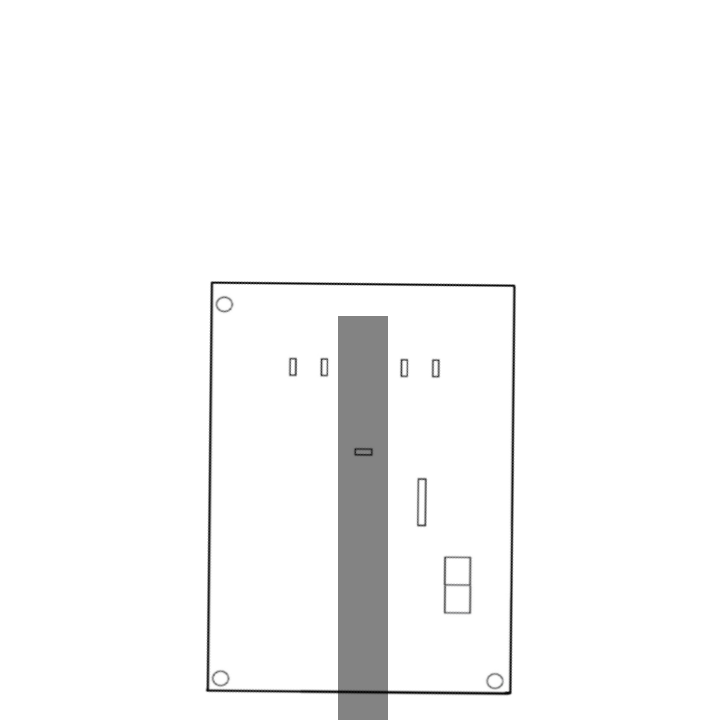
\includegraphics[width=0.2\textwidth]{figures/deadend1.png}
\caption{Center sensor polling for dead end.}
\end{figure}

\begin{figure}[H]
\centering
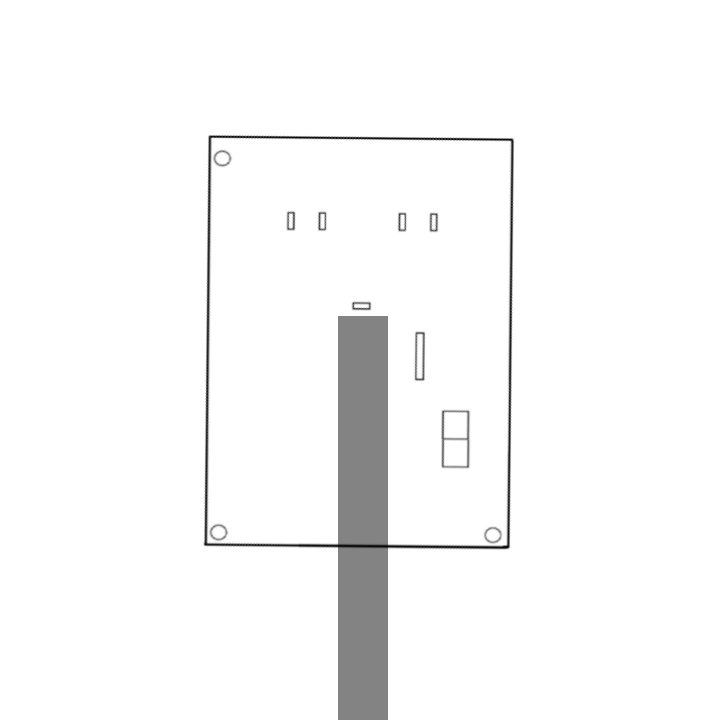
\includegraphics[width=0.2\textwidth]{figures/deadend2.png}
\caption{Center sensor detects event. Dead end inferred from internal logic.}
\end{figure}

\begin{figure}[H]
\centering
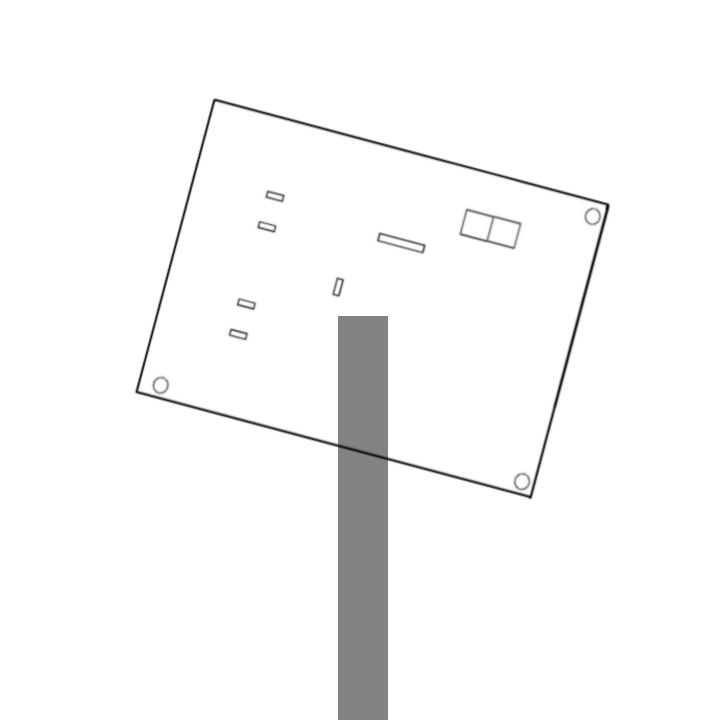
\includegraphics[width=0.2\textwidth]{figures/deadend3.png}
\caption{Robot begins turning here.}
\end{figure}

\begin{figure}[H]
\centering
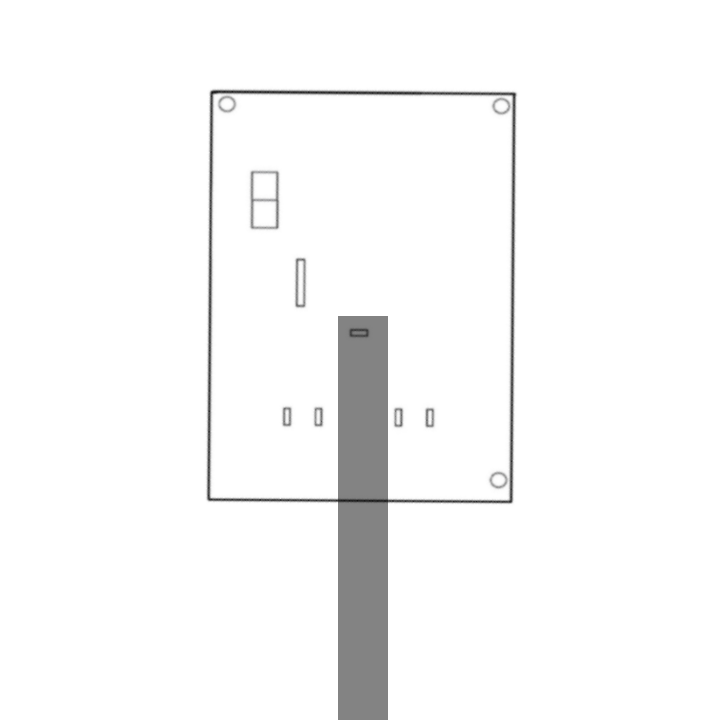
\includegraphics[width=0.2\textwidth]{figures/deadend4.png}
\caption{Robot completes 180 degree turn.}
\end{figure}

\end{multicols}

\subsection*{Appendix: E}

\begin{figure}[H]
\centering
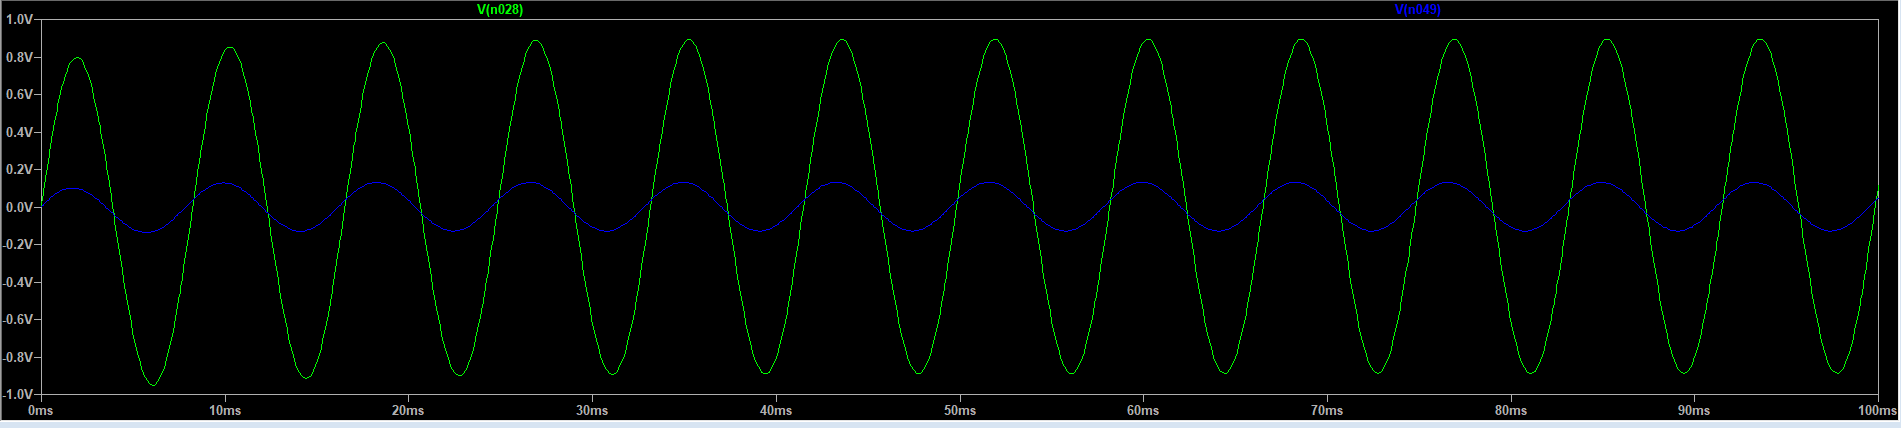
\includegraphics[width=\textwidth]{figures/LTS-filter.PNG}
\caption{LTSpice simulation of the high-pass filter component of the Active high-pass filter.}
\end{figure}

\begin{figure}[H]
\centering
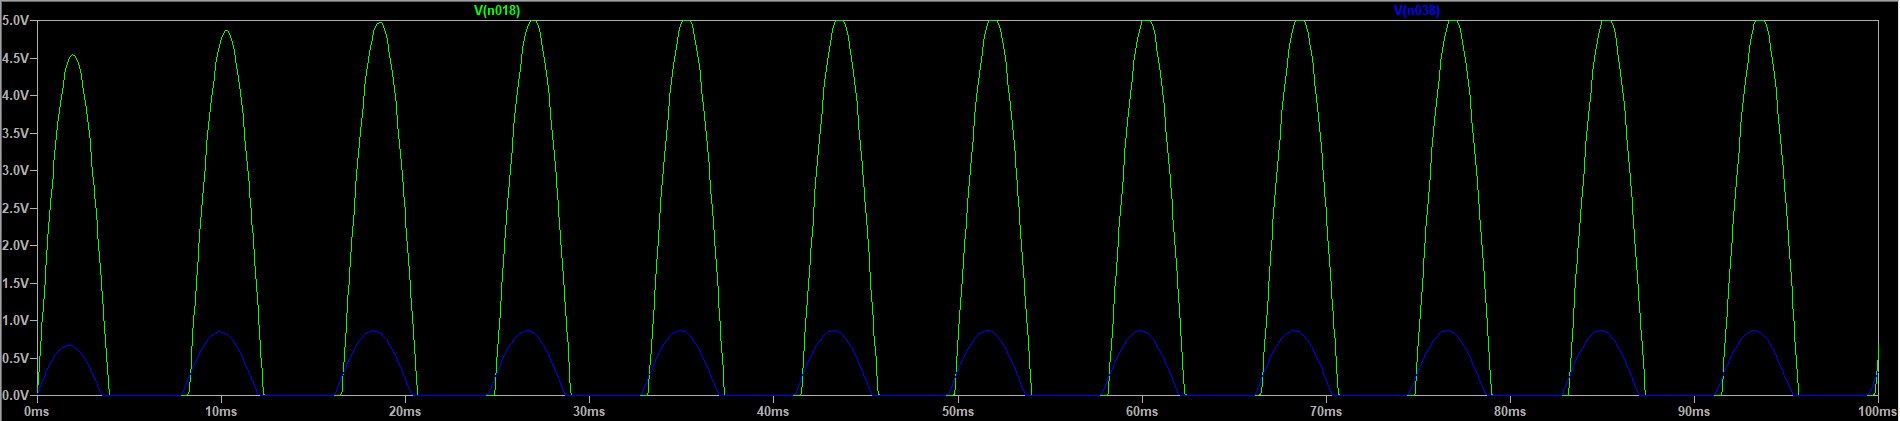
\includegraphics[width=\textwidth]{figures/LTS-gain.PNG}
\caption{LTSpice simulation of the amplification component of the Active high-pass filter.}
\end{figure}

\begin{figure}[H]
\centering
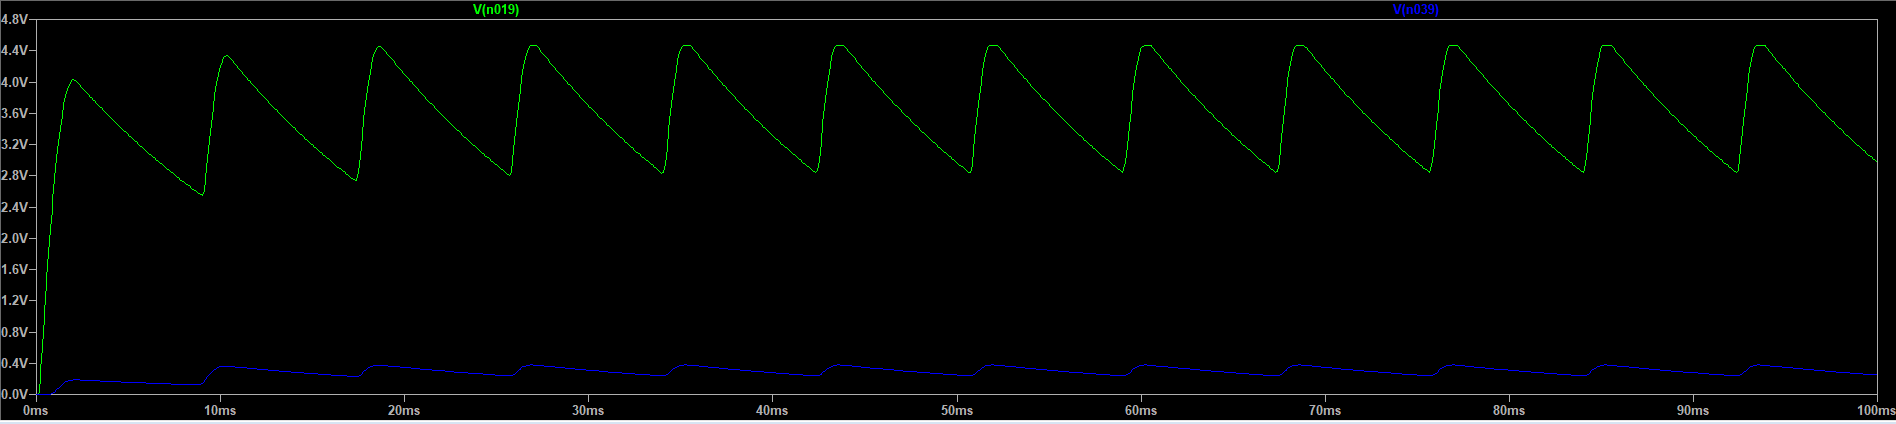
\includegraphics[width=\textwidth]{figures/LTS-rectified.PNG}
\caption{LTSpice simulation of the rectifier and smoothing capacitor output.}
\end{figure}

\begin{figure}[H]
\centering
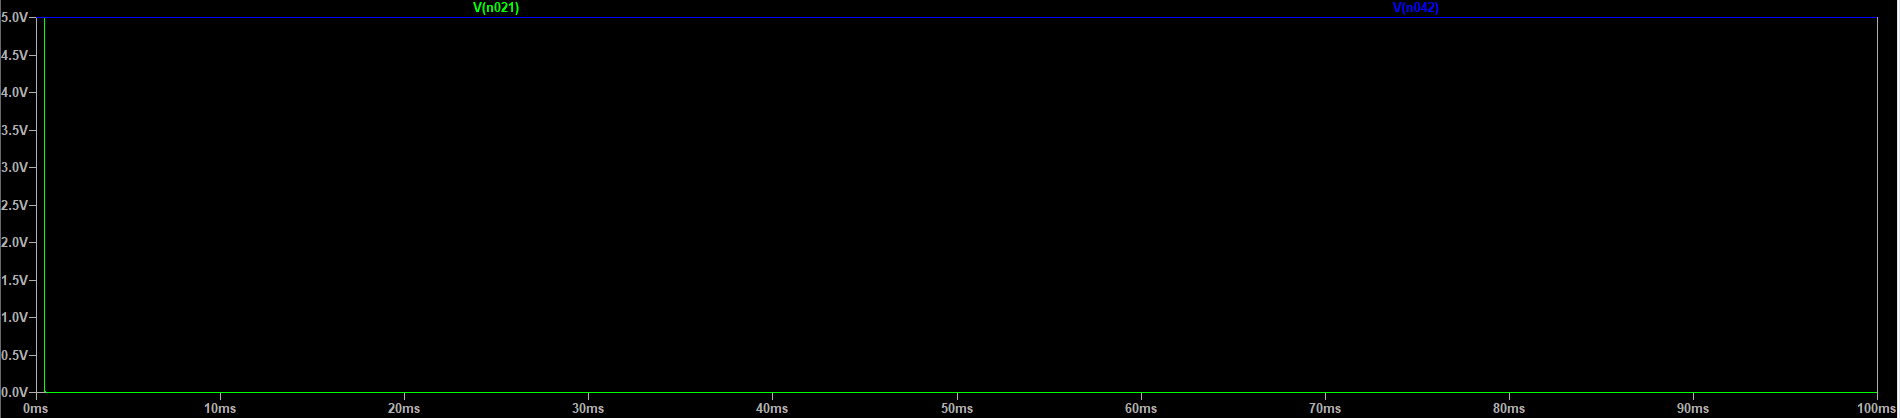
\includegraphics[width=\textwidth]{figures/LTS-output.PNG}
\caption{LTSpice simulation of the Schmitt-trigger output.}
\end{figure}

\begin{figure}[H]
\centering
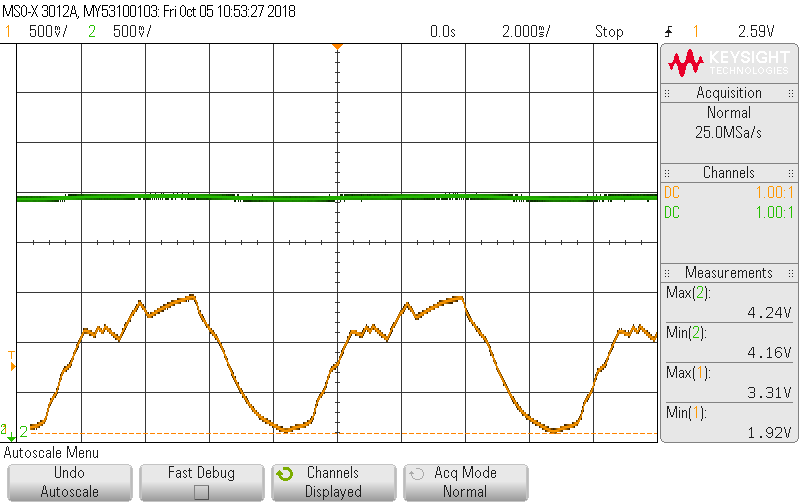
\includegraphics[width=0.9\textwidth]{figures/Osc-ls.png}
\caption{Light sensor output comparison between black and white light.}
\end{figure}

\begin{figure}[H]
\centering
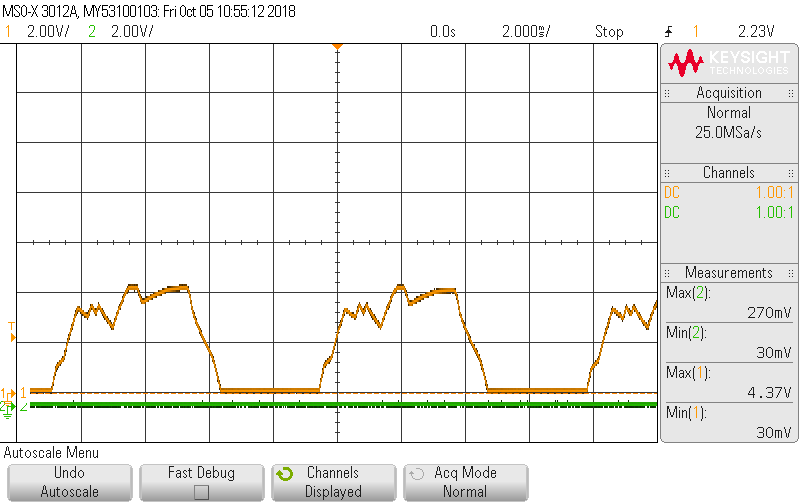
\includegraphics[width=0.9\textwidth]{figures/Osc-filtergain.png}
\caption{Active high-pass filter output comparison between black and white light.}
\end{figure}

\begin{figure}[H]
\centering
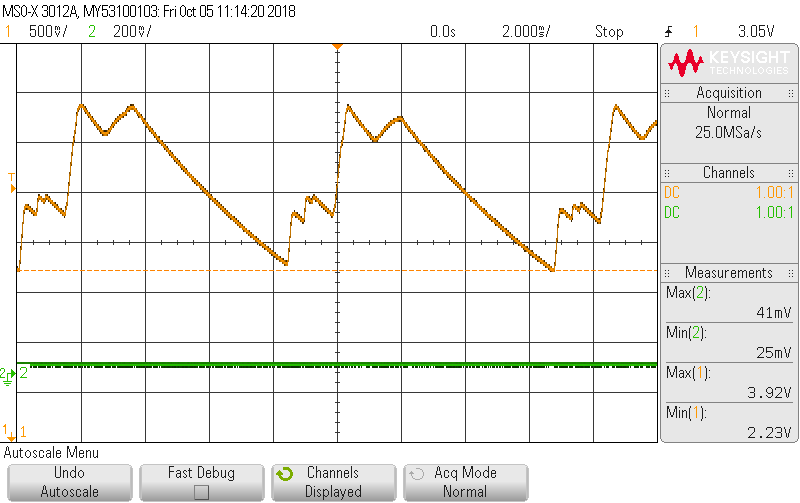
\includegraphics[width=0.9\textwidth]{figures/Osc-rectified.png}
\caption{Rectifier output comparison between black and white light.}
\end{figure}

\begin{figure}[H]
\centering
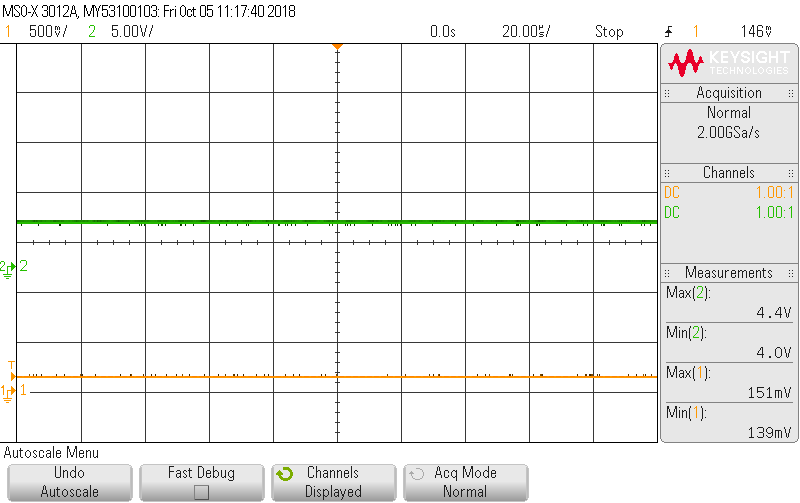
\includegraphics[width=0.9\textwidth]{figures/Osc-out.png}
\caption{Schmitt-trigger output comparison between black and white light.}
\end{figure}

\subsection*{Appendix: F}

\begin{figure}[H]
\centering
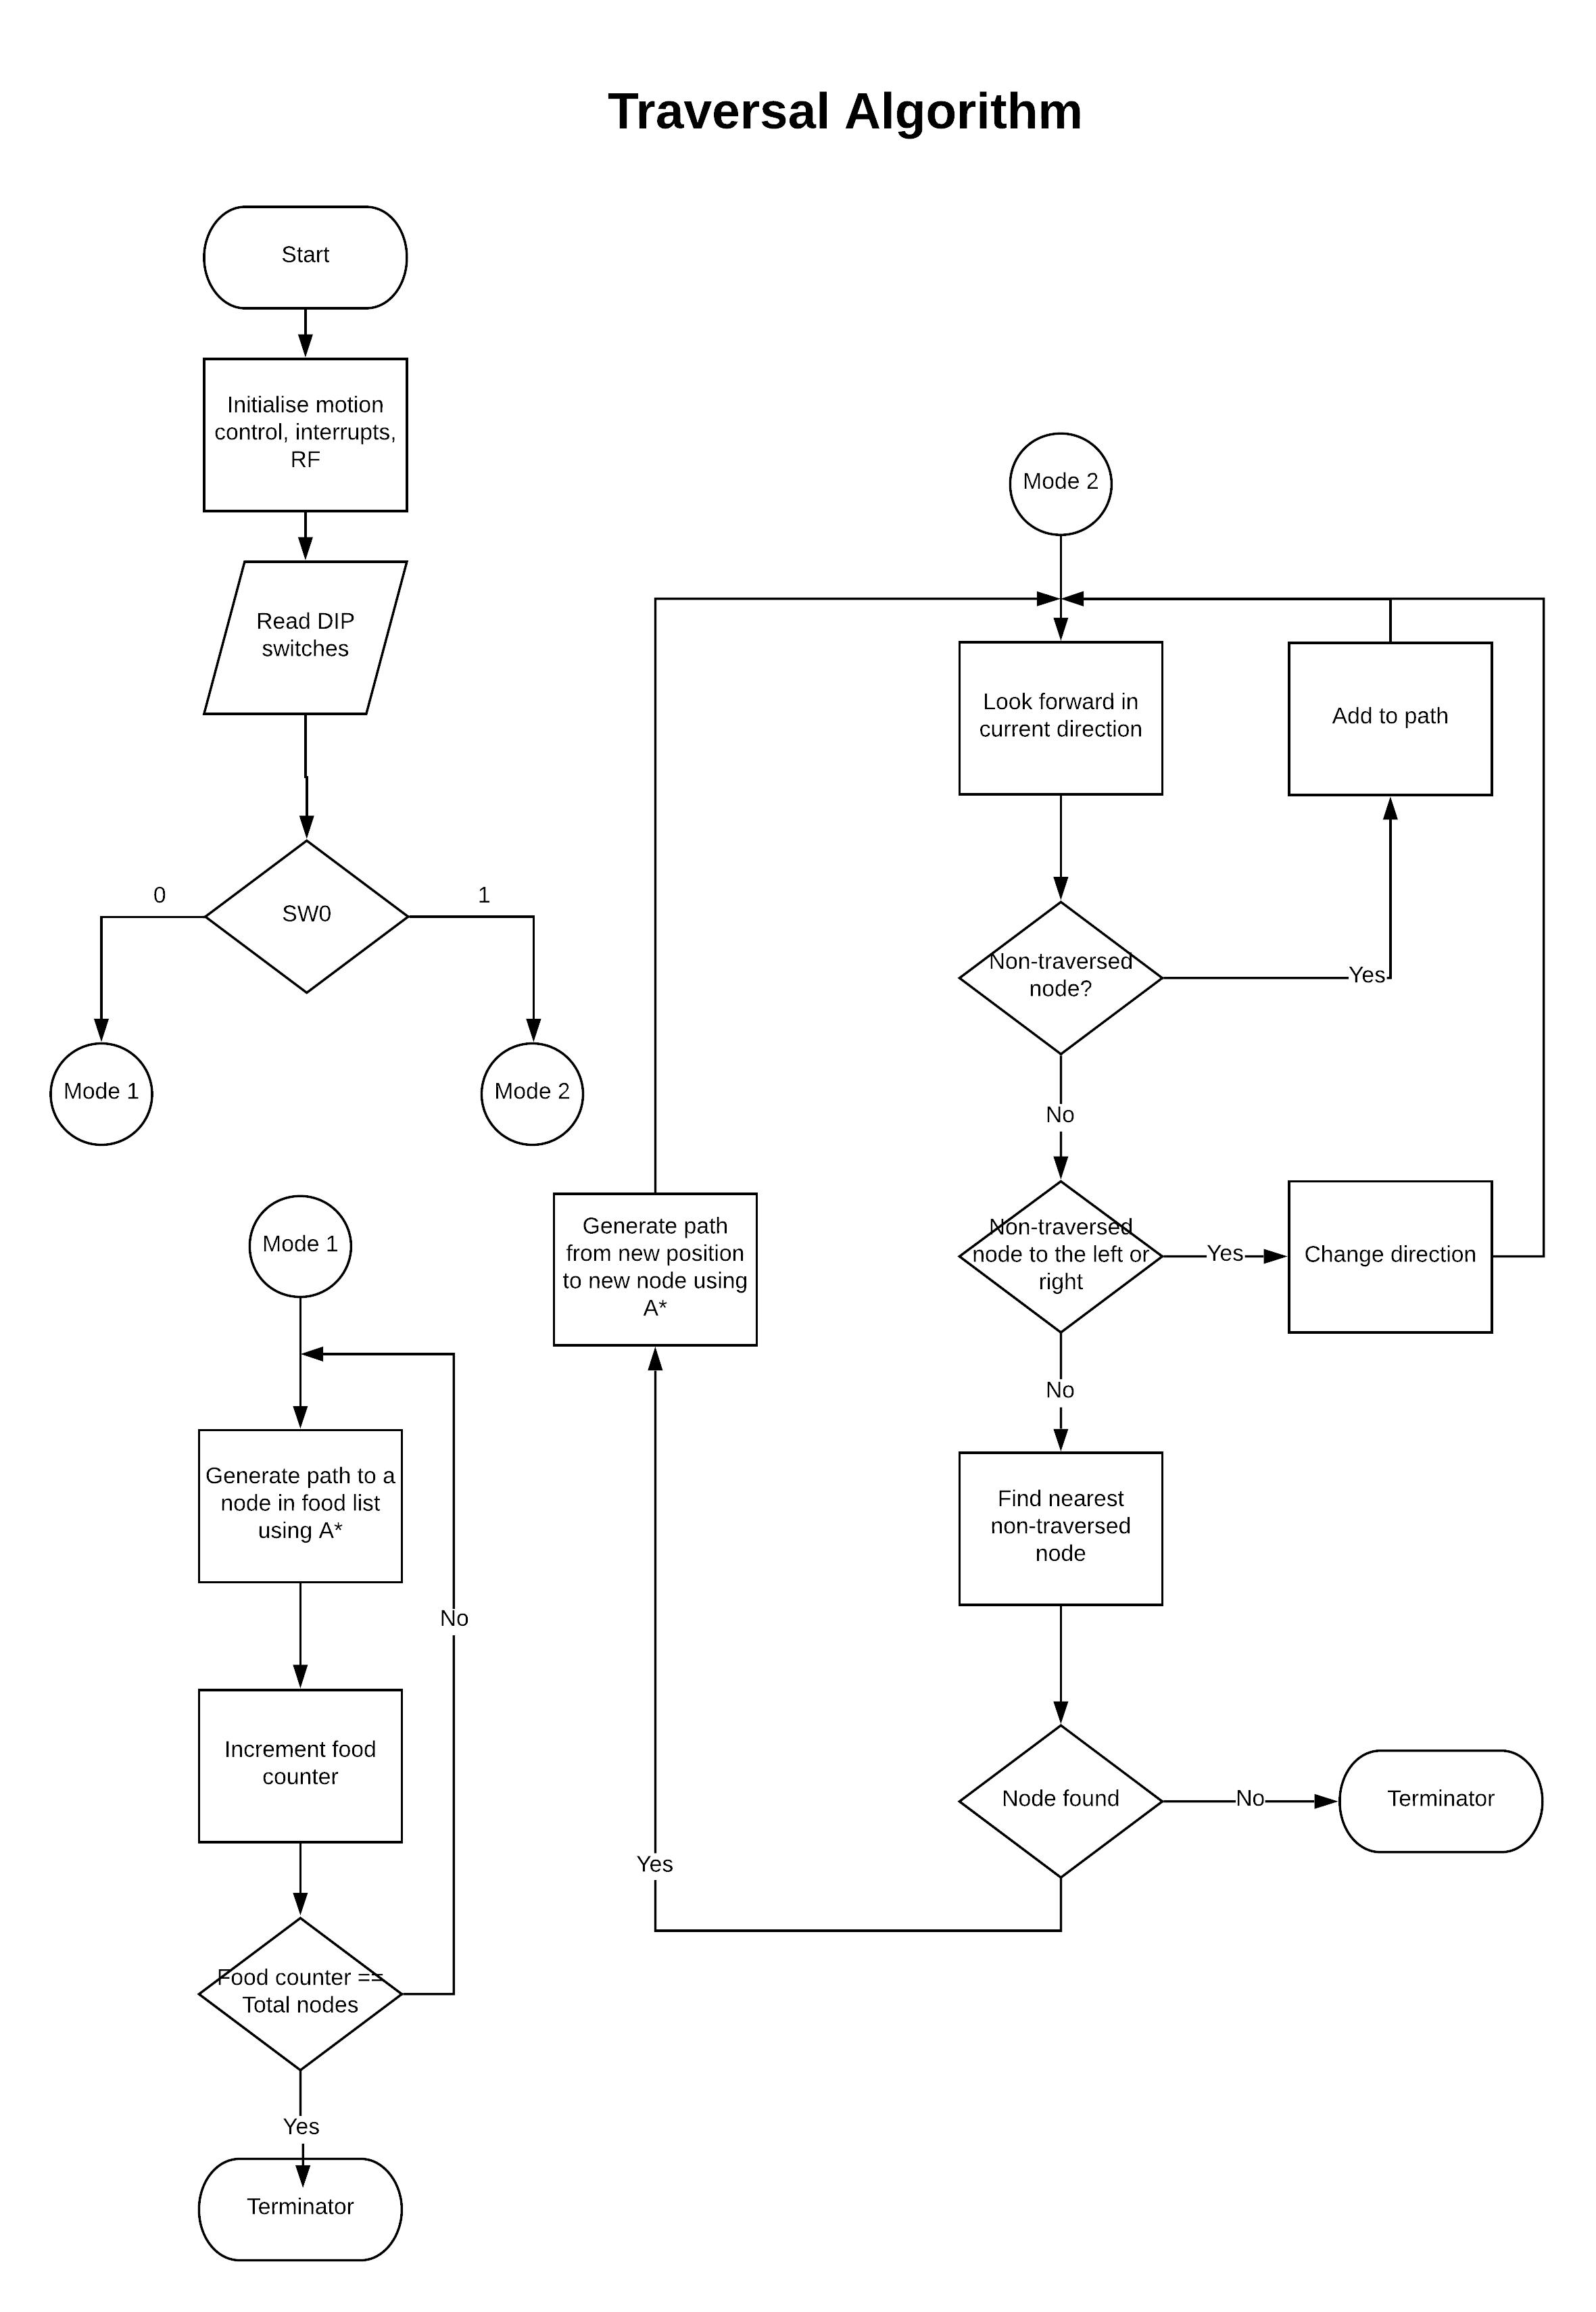
\includegraphics[width=0.8\textwidth]{figures/traverse_flowchart.png}
\caption{Traversal Algorithm Flowchart.}
\end{figure}

\begin{figure}[H]
\centering
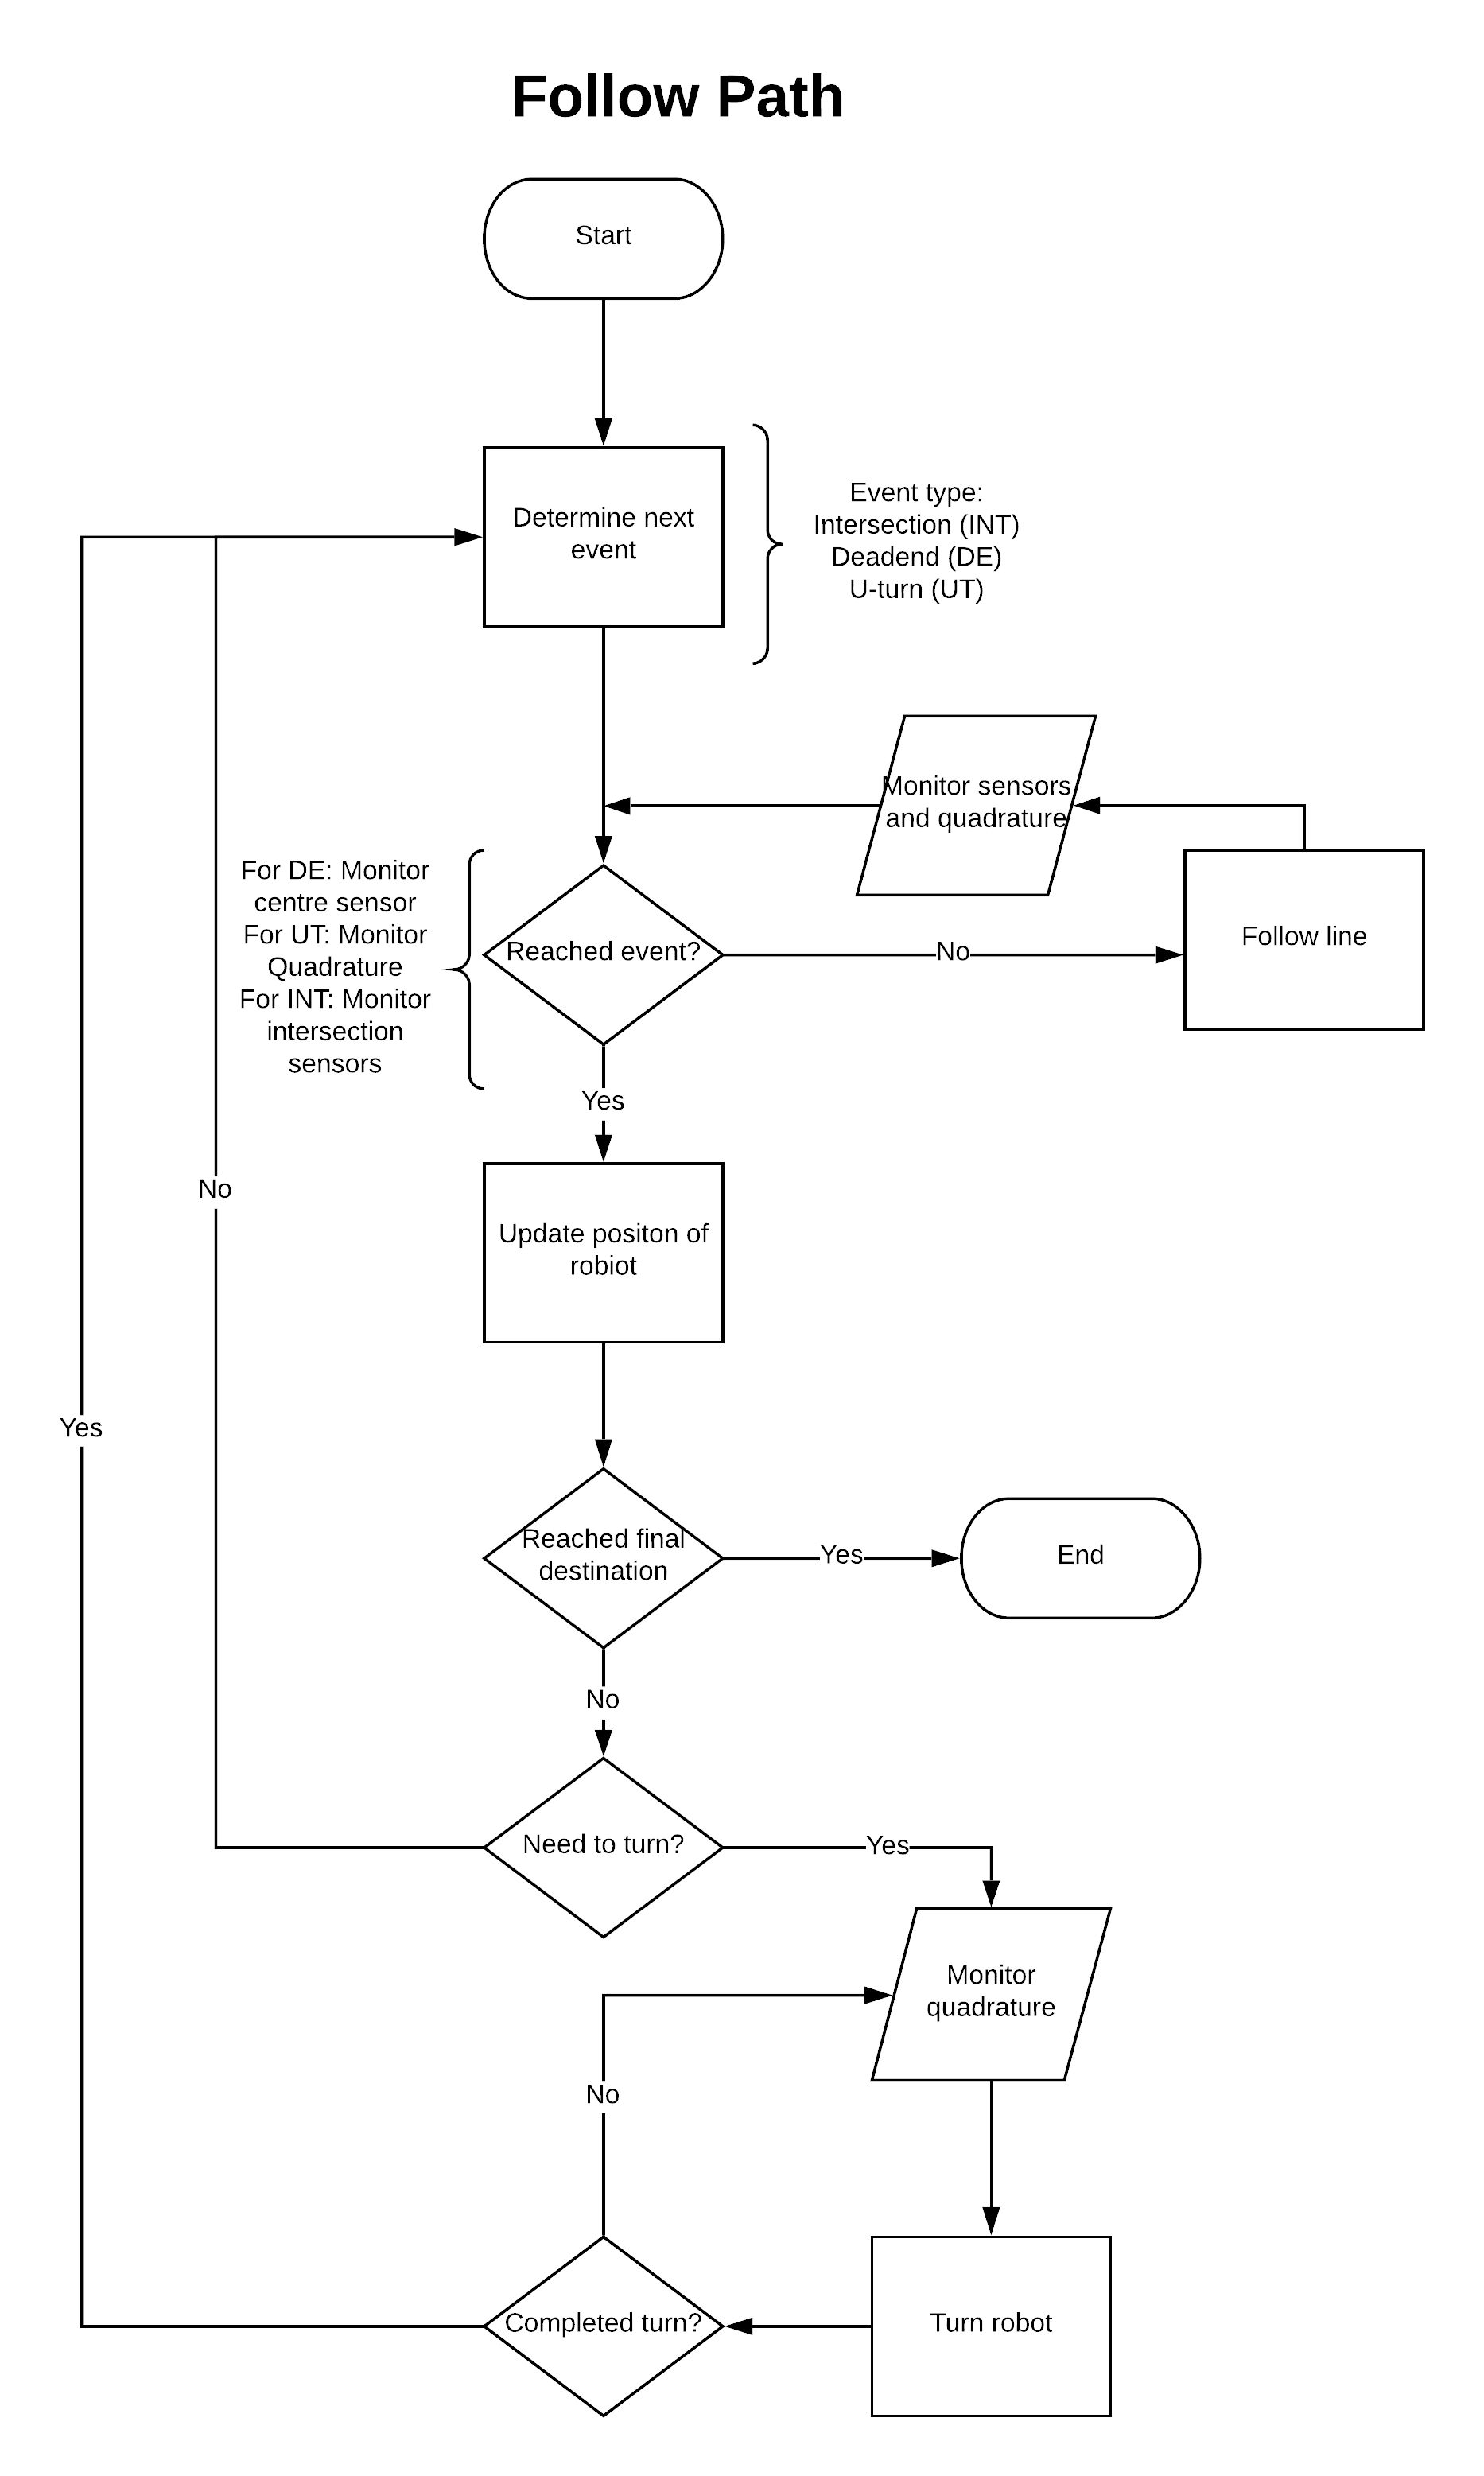
\includegraphics[width=0.7\textwidth]{figures/followpath_flowchart.png}
\caption{Follow Path Flowchart.}
\end{figure}

\begin{figure}[H]
\centering
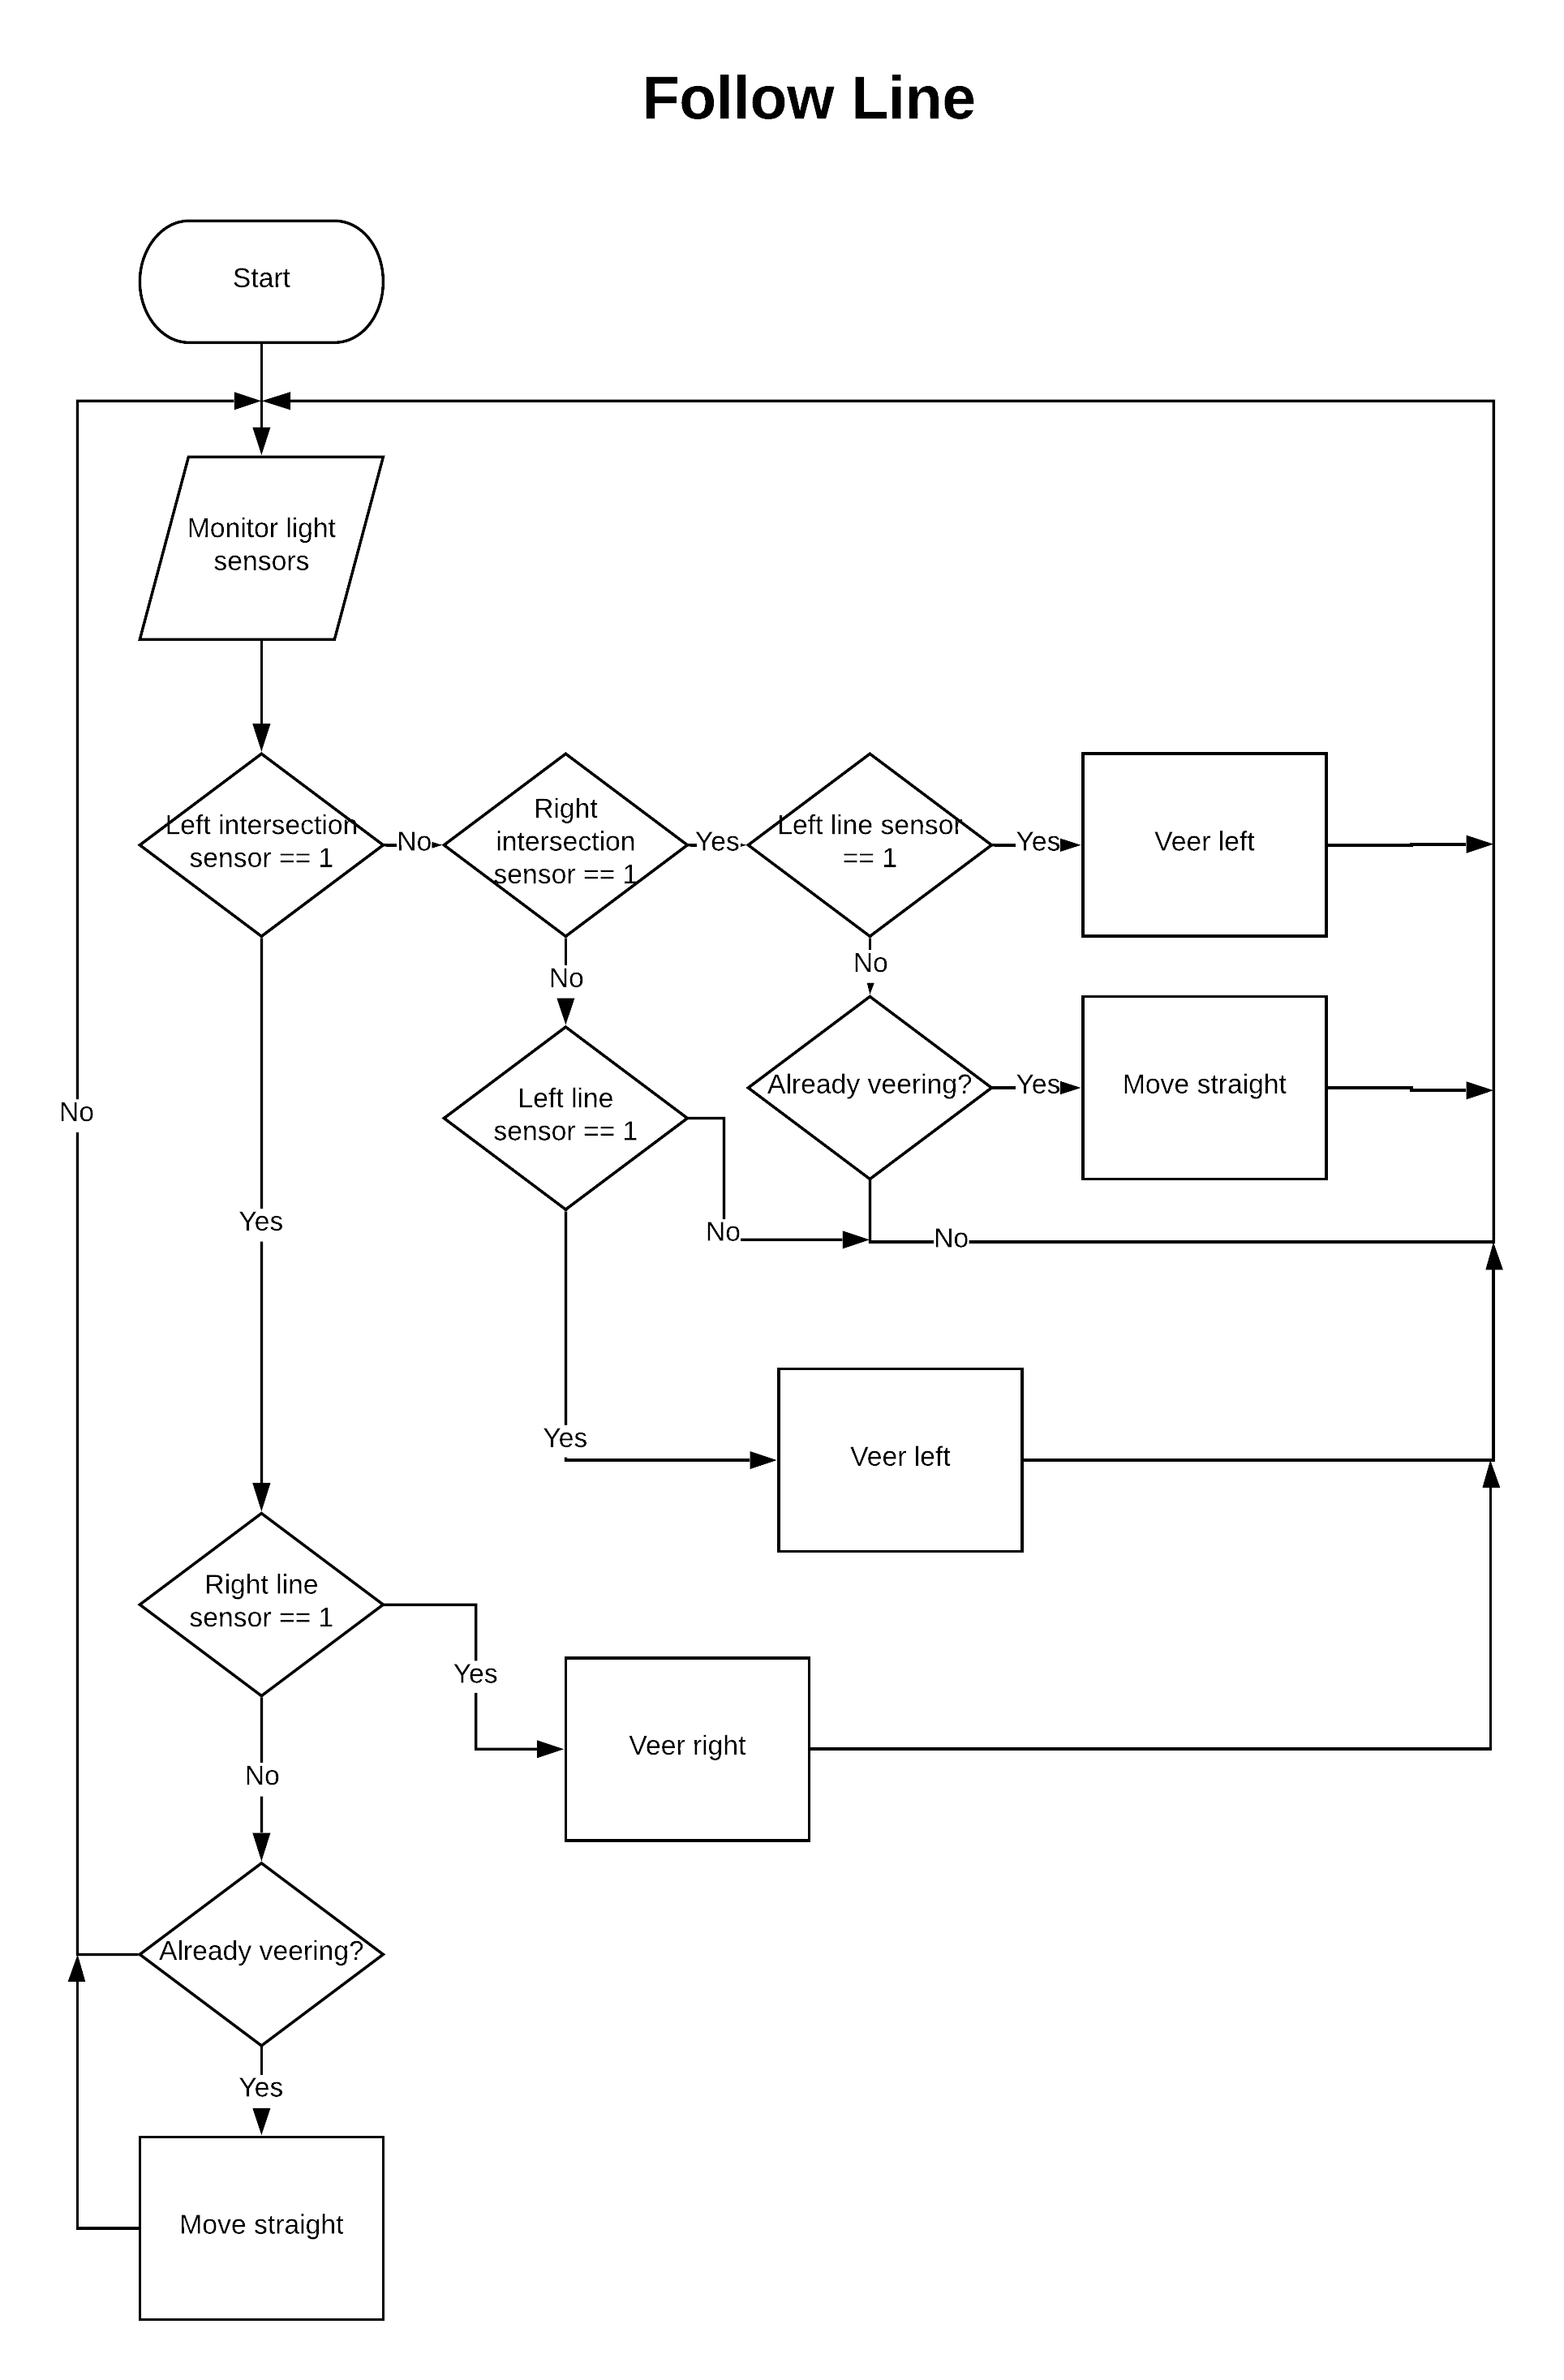
\includegraphics[width=0.8\textwidth]{figures/followline_flowchart.png}
\caption{Follow Line Flowchart.}
\end{figure}

\begin{figure}[H]
\centering
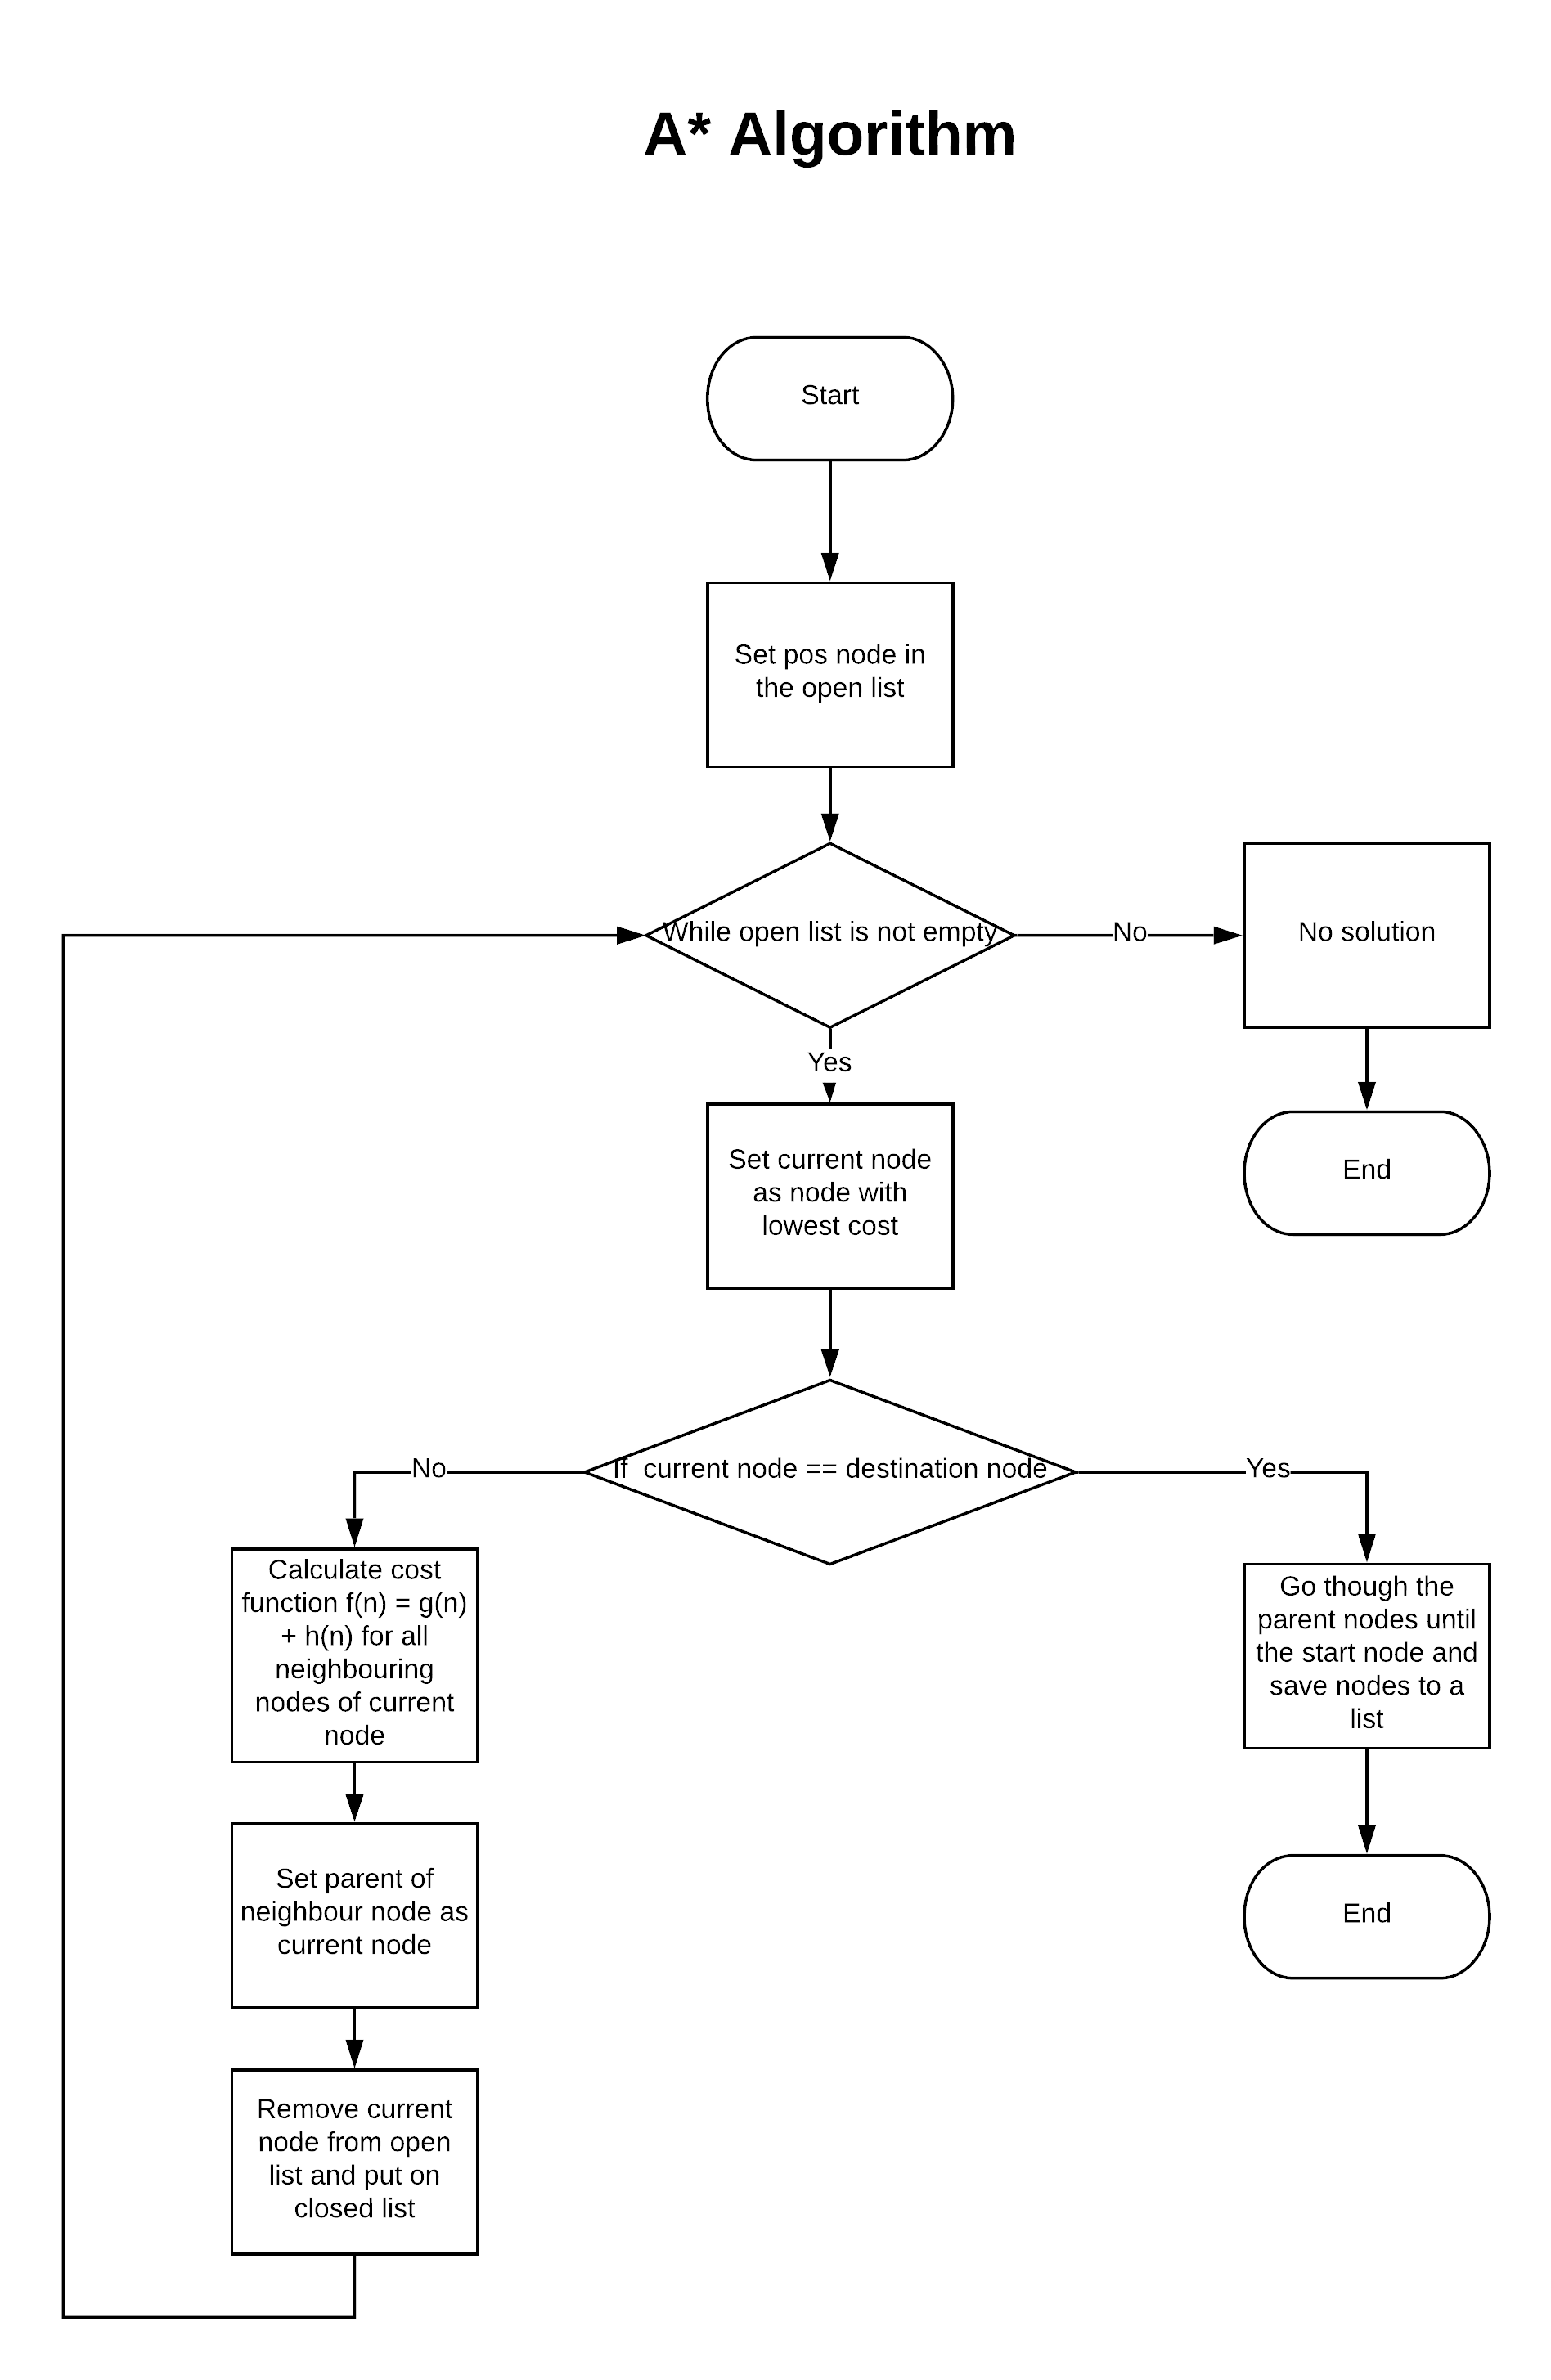
\includegraphics[width=0.8\textwidth]{figures/astar_flowchart.png}
\caption{A* Star Algorithm Flowchart.}
\end{figure}